\section{Metodologia}

É importante que se destaque a classificação de cada escolha metodológica realizada para a configuração deste trabalho. A Figura \ref{fig:classificacaoMetodologica}  apresenta esta classificação.

        \begin{figure}[h]
          \centering
          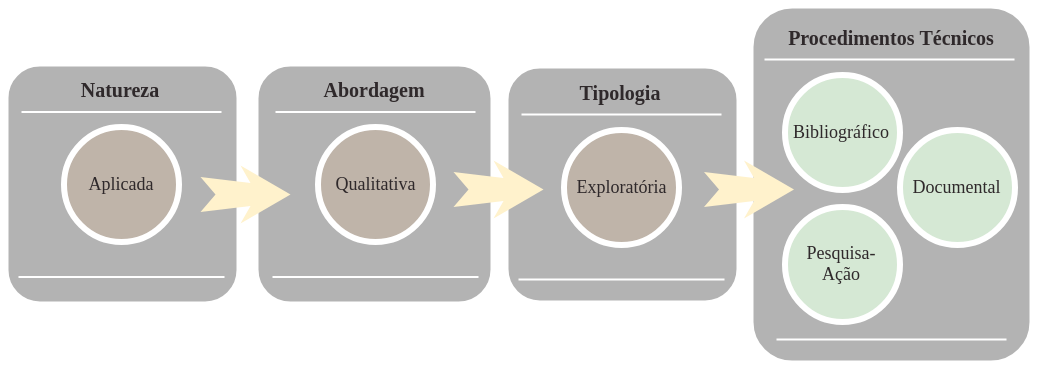
\includegraphics[width=14cm]{figuras/classificacaoMetodologica.png}
          \caption{Classificação Metodológica. (Fonte: Elaborado pela Autora.)} 
          \label{fig:classificacaoMetodologica}
        
        \end{figure}


Dado o contexto prático, no qual o objetivo é a criação de um módulo de uma ferramenta que promoverá a recomendação de \textit{tours} de Teste Exploratório baseado no perfil do testador, esta pesquisa é de natureza aplicada. A abordagem é qualitativa e quantitativa, uma vez que a análise dos dados fará uso de métodos e técnicas estatísticas.

Quanto ao tipo/objetivo, a pesquisa é classificada como explicativa, que possibilita a identificação de fatores que contribuem ou determinam a ocorrência de fenômenos,de modo a aprofundar o conhecimento da realidade e a explicar a razão e motivo das coisas~\cite{gil2002elaborar}. 

Dado que se busca criar um módulo em uma ferramenta, neste trabalho adotou-se a técnica de pesquisa-ação, que possibilita
ao pesquisador a construção de instrumentos em ciclos de iteração com a equipe, isso é, entre os pesquisadores e a organização alvo de estudos. Dessa forma, será possível a construção da ferramenta em ciclos de interação com o refinamento e validação do algoritmo de recomendação de \textit{tours} baseado em cada perfil de testador.

A Pesquisa-ação, proposta por~\cite{petersen2008systematic} é empregad com as etapas Diagnóstico, Planejamento da ação, Reflexão e Tomada de decisão, cujo objetivo é a realização de ciclos de iteração para a especificação de um instrumento; seguida da técnica Estudo de Caso empregada na Construção do instrumento, cujo objetivo é desenvolver um sistema a partir da especificação definida de forma iterativa na fase anterior, como demonstrado na Figura \ref{fig:etapasPesquisaAcaoAdotas}.

        \begin{figure}[H]
          \centering
          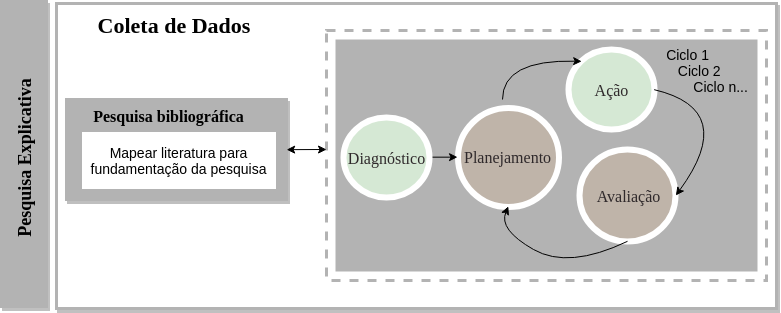
\includegraphics[width=12cm]{figuras/etapasPesquisaAcaoAdotadas.png}
          \caption{Etapas da Pesquisa-Ação adotadas. (Fonte: Elaborado pela Autora.)} 
          \label{fig:etapasPesquisaAcaoAdotas}
        
        \end{figure}

O plano metodológico adotado neste trabalho compreendeu quatro fases básicas: \textit{planejamento da pesquisa}; \textit{coleta de dados}; \textit{análise dos dados}; e \textit{relato dos resultados}. O detalhamento deste planejamento metodológico encontra-se no Capítulo Materiais e Métodos.


